% Options for packages loaded elsewhere
% Options for packages loaded elsewhere
\PassOptionsToPackage{unicode}{hyperref}
\PassOptionsToPackage{hyphens}{url}
%
\documentclass[
  ignorenonframetext,
  aspectratio=169,
]{beamer}
\newif\ifbibliography
\usepackage{pgfpages}
\setbeamertemplate{caption}[numbered]
\setbeamertemplate{caption label separator}{: }
\setbeamercolor{caption name}{fg=normal text.fg}
\beamertemplatenavigationsymbolsempty
% remove section numbering
\setbeamertemplate{part page}{
  \centering
  \begin{beamercolorbox}[sep=16pt,center]{part title}
    \usebeamerfont{part title}\insertpart\par
  \end{beamercolorbox}
}
\setbeamertemplate{section page}{
  \centering
  \begin{beamercolorbox}[sep=12pt,center]{section title}
    \usebeamerfont{section title}\insertsection\par
  \end{beamercolorbox}
}
\setbeamertemplate{subsection page}{
  \centering
  \begin{beamercolorbox}[sep=8pt,center]{subsection title}
    \usebeamerfont{subsection title}\insertsubsection\par
  \end{beamercolorbox}
}
% Prevent slide breaks in the middle of a paragraph
\widowpenalties 1 10000
\raggedbottom
\usepackage{iftex}
\ifPDFTeX
  \usepackage[T1]{fontenc}
  \usepackage[utf8]{inputenc}
  \usepackage{textcomp} % provide euro and other symbols
\else % if luatex or xetex
  \usepackage{unicode-math} % this also loads fontspec
  \defaultfontfeatures{Scale=MatchLowercase}
  \defaultfontfeatures[\rmfamily]{Ligatures=TeX,Scale=1}
\fi
\usepackage{lmodern}

\usetheme[]{metropolis}
\ifPDFTeX\else
  % xetex/luatex font selection
\fi
% Use upquote if available, for straight quotes in verbatim environments
\IfFileExists{upquote.sty}{\usepackage{upquote}}{}
\IfFileExists{microtype.sty}{% use microtype if available
  \usepackage[]{microtype}
  \UseMicrotypeSet[protrusion]{basicmath} % disable protrusion for tt fonts
}{}
\makeatletter
\@ifundefined{KOMAClassName}{% if non-KOMA class
  \IfFileExists{parskip.sty}{%
    \usepackage{parskip}
  }{% else
    \setlength{\parindent}{0pt}
    \setlength{\parskip}{6pt plus 2pt minus 1pt}}
}{% if KOMA class
  \KOMAoptions{parskip=half}}
\makeatother


\usepackage{longtable,booktabs,array}
\usepackage{calc} % for calculating minipage widths
\usepackage{caption}
% Make caption package work with longtable
\makeatletter
\def\fnum@table{\tablename~\thetable}
\makeatother
\usepackage{graphicx}
\makeatletter
\newsavebox\pandoc@box
\newcommand*\pandocbounded[1]{% scales image to fit in text height/width
  \sbox\pandoc@box{#1}%
  \Gscale@div\@tempa{\textheight}{\dimexpr\ht\pandoc@box+\dp\pandoc@box\relax}%
  \Gscale@div\@tempb{\linewidth}{\wd\pandoc@box}%
  \ifdim\@tempb\p@<\@tempa\p@\let\@tempa\@tempb\fi% select the smaller of both
  \ifdim\@tempa\p@<\p@\scalebox{\@tempa}{\usebox\pandoc@box}%
  \else\usebox{\pandoc@box}%
  \fi%
}
% Set default figure placement to htbp
\def\fps@figure{htbp}
\makeatother





\setlength{\emergencystretch}{3em} % prevent overfull lines

\providecommand{\tightlist}{%
  \setlength{\itemsep}{0pt}\setlength{\parskip}{0pt}}



 


% ============================================================
%  Econ 2203 — Beamer Metropolis Theme Preamble
%  Course: International Trade and Policy in Agriculture
%  Instructor: Nithin M, Department of Development Economics
% ============================================================

% MUST be first: load Metropolis theme before \metroset and colour overrides
\usetheme{metropolis}

% Only load packages not already provided by pandoc's beamer template
\usepackage{amsmath,amssymb}

% ---- Brand colours -----------------------------------------
\definecolor{brandblue}{HTML}{012169}
\definecolor{brandgold}{HTML}{B9975B}
\definecolor{lightblue}{HTML}{E8EDF5}

% ---- Metropolis colour overrides ---------------------------
% Main palette
\setbeamercolor{normal text}{fg=black,bg=white}
\setbeamercolor{alerted text}{fg=brandgold}
\setbeamercolor{example text}{fg=brandblue!70!black}

% Title slide
\setbeamercolor{title}{fg=white,bg=brandblue}
\setbeamercolor{subtitle}{fg=brandgold}
\setbeamercolor{author}{fg=white}
\setbeamercolor{institute}{fg=brandgold!80!white}
\setbeamercolor{date}{fg=white}
\setbeamercolor{title page header}{fg=white,bg=brandblue}

% Frametitle bar
\setbeamercolor{frametitle}{fg=white,bg=brandblue}

% Progress bar → gold
\setbeamercolor{progress bar}{fg=brandgold,bg=brandblue!30}
\setbeamercolor{title separator}{fg=brandgold}
\setbeamercolor{progress bar in head/foot}{fg=brandgold,bg=brandblue!20}
\setbeamercolor{progress bar in section page}{fg=brandgold,bg=brandblue!20}

% Blocks
\setbeamercolor{block title}{bg=brandblue,fg=white}
\setbeamercolor{block body}{bg=lightblue,fg=black}
\setbeamercolor{block title alerted}{bg=brandgold,fg=white}
\setbeamercolor{block body alerted}{bg=brandgold!12,fg=black}
\setbeamercolor{block title example}{bg=brandblue!70!black,fg=white}
\setbeamercolor{block body example}{bg=brandblue!8,fg=black}

% Structure / lists
\setbeamercolor{structure}{fg=brandblue}
\setbeamercolor{section in toc}{fg=brandblue}
\setbeamercolor{itemize item}{fg=brandblue}
\setbeamercolor{itemize subitem}{fg=brandgold}
\setbeamercolor{enumerate item}{fg=brandblue}
\setbeamercolor{description item}{fg=brandblue}

% ---- Metropolis options ------------------------------------
\metroset{
  progressbar    = frametitle,   % gold bar under frametitle
  sectionpage    = none,
  numbering      = fraction,
  block          = fill
}

% ---- Fonts (Metropolis uses Fira Sans; fallback gracefully) -
\setbeamerfont{title}{size=\Large,series=\bfseries}
\setbeamerfont{subtitle}{size=\normalsize,series=\mdseries}
\setbeamerfont{frametitle}{size=\large,series=\bfseries}
\setbeamerfont{block title}{size=\normalsize,series=\bfseries}
\setbeamerfont{caption}{size=\footnotesize}

% ---- Footer: course info + slide number --------------------
\setbeamertemplate{footline}{%
  \begin{beamercolorbox}[wd=\paperwidth,ht=2.0ex,dp=1ex]{footline}%
    \hspace{0.8em}%
    {\footnotesize\color{brandblue!60}%
      Econ 2203 \textbar{} International Trade and Policy in Agriculture
      \hfill Nithin M \hfill
      \insertframenumber{}/\inserttotalframenumber\hspace{0.8em}}%
  \end{beamercolorbox}%
}

% ---- Misc --------------------------------------------------
\setlength{\parskip}{0.25em}
\setbeamertemplate{navigation symbols}{}

% tighter column sep for side-by-side content
\setlength{\columnsep}{0.8em}

% Fix: make \label truly robust in moving arguments (Quarto generates
% \caption{\label{fig-xxx}...} which crashes Metropolis in batchmode).
% DeclareRobustCommand creates a self-protecting robust version.
\makeatletter
\let\quarto@originallabel\label
\DeclareRobustCommand*{\label}[1]{\quarto@originallabel{#1}}
\makeatother

% Prevent figures from overflowing Beamer frames.
% width=\linewidth: scale to text width (already Quarto default);
% height=0.6\textheight: cap height so figures never push past the frame bottom.
% keepaspectratio: never distort — whichever constraint binds first wins.
\setkeys{Gin}{width=\linewidth,height=0.6\textheight,keepaspectratio}
\makeatletter
\@ifpackageloaded{caption}{}{\usepackage{caption}}
\AtBeginDocument{%
\ifdefined\contentsname
  \renewcommand*\contentsname{Table of contents}
\else
  \newcommand\contentsname{Table of contents}
\fi
\ifdefined\listfigurename
  \renewcommand*\listfigurename{List of Figures}
\else
  \newcommand\listfigurename{List of Figures}
\fi
\ifdefined\listtablename
  \renewcommand*\listtablename{List of Tables}
\else
  \newcommand\listtablename{List of Tables}
\fi
\ifdefined\figurename
  \renewcommand*\figurename{Figure}
\else
  \newcommand\figurename{Figure}
\fi
\ifdefined\tablename
  \renewcommand*\tablename{Table}
\else
  \newcommand\tablename{Table}
\fi
}
\@ifpackageloaded{float}{}{\usepackage{float}}
\floatstyle{ruled}
\@ifundefined{c@chapter}{\newfloat{codelisting}{h}{lop}}{\newfloat{codelisting}{h}{lop}[chapter]}
\floatname{codelisting}{Listing}
\newcommand*\listoflistings{\listof{codelisting}{List of Listings}}
\makeatother
\makeatletter
\makeatother
\makeatletter
\@ifpackageloaded{caption}{}{\usepackage{caption}}
\@ifpackageloaded{subcaption}{}{\usepackage{subcaption}}
\makeatother

\usepackage{bookmark}
\IfFileExists{xurl.sty}{\usepackage{xurl}}{} % add URL line breaks if available
\urlstyle{same}
\hypersetup{
  pdftitle={Lecture 13: WTO --- Origin, Structure and Functions},
  pdfauthor={Nithin M},
  hidelinks,
  pdfcreator={LaTeX via pandoc}}


\title{Lecture 13: WTO --- Origin, Structure and Functions}
\subtitle{Econ 2203 \textbar{} International Trade and Policy in
Agriculture}
\author{Nithin M}
\date{2026-07-18}
\institute{Department of Development Economics}

\begin{document}
\frame{\titlepage}


\begin{frame}{Recap: Lecture 12}
\phantomsection\label{recap-lecture-12}
\textbf{Lecture 12} examined the \textbf{foreign exchange market} ---
how currencies are priced, how the exchange rate affects export
competitiveness, and how India manages the rupee.

\begin{columns}[T]
\begin{column}{0.55\linewidth}
\textbf{Key ideas from Lecture 12:}

\begin{itemize}
\tightlist
\item
  Exchange rate as the price of international trade
\item
  Real exchange rate determines competitiveness
\item
  RBI intervention in the forex market
\item
  Currency depreciation ↑ export attractiveness
\end{itemize}
\end{column}

\begin{column}{0.45\linewidth}
\textbf{The Bridge to Today}

Trade actually happens through the forex system --- but \textbf{what
rules govern the trade itself?}

Who decides that a country cannot ban imports arbitrarily? Who enforces
fair competition?

→ Enter the \textbf{World Trade Organization}
\end{column}
\end{columns}
\end{frame}

\begin{frame}
\end{frame}

\section{From GATT to WTO}\label{from-gatt-to-wto}

\begin{frame}{GATT to WTO: A Brief History}
\phantomsection\label{gatt-to-wto-a-brief-history}
\begin{columns}[T]
\begin{column}{0.5\linewidth}
\textbf{General Agreement on Tariffs and Trade (1947)}

\begin{itemize}
\tightlist
\item
  Signed Oct 1947; entered into force Jan 1948
\item
  \textbf{23 original contracting parties} (provisional --- never
  ratified by US Congress)
\item
  Goal: reduce tariffs and quantitative restrictions
\item
  Eight negotiating rounds over 47 years:
\end{itemize}

\begin{longtable}[]{@{}lll@{}}
\toprule\noalign{}
Round & Year & Key Focus \\
\midrule\noalign{}
\endhead
Geneva & 1947 & Tariff cuts \\
Dillon & 1960--61 & Tariff cuts \\
Kennedy & 1964--67 & Tariff + anti-dumping \\
Tokyo & 1973--79 & NTBs \\
\textbf{Uruguay} & \textbf{1986--94} & \textbf{Agriculture, services,
WTO} \\
\bottomrule\noalign{}
\end{longtable}
\end{column}

\begin{column}{0.5\linewidth}
\textbf{Why GATT Failed Agriculture}

\textbf{Three critical weaknesses:}

\begin{enumerate}
\tightlist
\item
  \textbf{No enforcement} --- ``diplomatic'' dispute resolution, losing
  party could block adoption of panel report
\item
  \textbf{Agriculture excluded} --- US/EU ``waivers'' exempted farm
  support from discipline
\item
  \textbf{No services, no IP} --- growing share of world trade uncovered
\end{enumerate}

WTO replaced GATT on \textbf{January 1, 1995} as a permanent
international organisation with legal personality, headquarters in
Geneva.
\end{column}
\end{columns}
\end{frame}

\begin{frame}{The Uruguay Round (1986--1994)}
\phantomsection\label{the-uruguay-round-19861994}
\textbf{The most ambitious multilateral trade negotiation in history}
--- 8 years, 123 countries, launched in Punta del Este, Uruguay

\begin{columns}[T]
\begin{column}{0.5\linewidth}
\textbf{What was new:}

\begin{itemize}
\tightlist
\item
  🌾 \textbf{Agriculture} --- AoA for the first time
\item
  🏢 \textbf{Services} --- General Agreement on Trade in Services (GATS)
\item
  💡 \textbf{Intellectual Property} --- TRIPS Agreement
\item
  🔨 \textbf{Binding dispute settlement} --- no more blocking
\end{itemize}

\textbf{Signed at:} Marrakesh, Morocco --- \textbf{April 15, 1994}
(Marrakesh Agreement)

\textbf{India's role:} Active participant; founding WTO member
\end{column}

\begin{column}{0.5\linewidth}
\textbf{Uruguay Round Achievements}

\begin{itemize}
\tightlist
\item
  Tariff cuts on industrial goods: \textasciitilde40\%
\item
  Agriculture: brought under multilateral discipline for first time
\item
  Services: GATS framework established
\item
  Intellectual property: TRIPS agreement
\item
  Dispute settlement: binding DSU mechanism
\item
  WTO: permanent institution created
\item
  Single undertaking: all-or-nothing package
\end{itemize}

\textbf{Single Undertaking Principle:} ``Nothing is agreed until
everything is agreed'' --- countries had to accept the entire package,
preventing cherry-picking.
\end{column}
\end{columns}
\end{frame}

\begin{frame}{Global Trade vs GDP Growth Index}
\phantomsection\label{global-trade-vs-gdp-growth-index}
\begin{figure}

\centering{

\pandocbounded{
\includegraphics[keepaspectratio]{Lecture13_WTO_files/figure-beamer/fig-trade-gdp-1.pdf}}

}

\caption{\label{fig-trade-gdp}Global Trade vs GDP Growth Index
(2000-2023) Source: WTO, World Trade Statistical Review 2024; World
Bank, WDI.}

\end{figure}%
\end{frame}

\begin{frame}{WTO at a Glance}
\phantomsection\label{wto-at-a-glance}
\begin{columns}[T]
\begin{column}{0.5\linewidth}
\textbf{Key Facts (2024)}

\begin{longtable}[]{@{}ll@{}}
\toprule\noalign{}
Item & Detail \\
\midrule\noalign{}
\endhead
Headquarters & Geneva, Switzerland \\
Members & \textbf{166} (as of 2024) \\
Founded & January 1, 1995 \\
India & \textbf{Founding member} \\
Budget & \textasciitilde CHF 197 million/year \\
Staff & \textasciitilde700 \\
Official languages & English, French, Spanish \\
\bottomrule\noalign{}
\end{longtable}

\textbf{Two-thirds of members are developing countries} --- WTO is not a
``rich country club''
\end{column}

\begin{column}{0.5\linewidth}
\textbf{Director-General:}

\textbf{Ngozi Okonjo-Iweala} (Since February 1, 2021)

\begin{itemize}
\tightlist
\item
  First \textbf{woman} DG in WTO history
\item
  First \textbf{African} DG in WTO history
\item
  Former Finance Minister of Nigeria
\item
  Former World Bank Managing Director
\end{itemize}

Re-appointed for second term (2025--2029)

India has been a founding and \textbf{strategically active} member ---
one of the most influential developing country voices at the WTO
\end{column}
\end{columns}
\end{frame}

\begin{frame}{WTO Membership Growth}
\phantomsection\label{wto-membership-growth}
\begin{figure}

\centering{

\pandocbounded{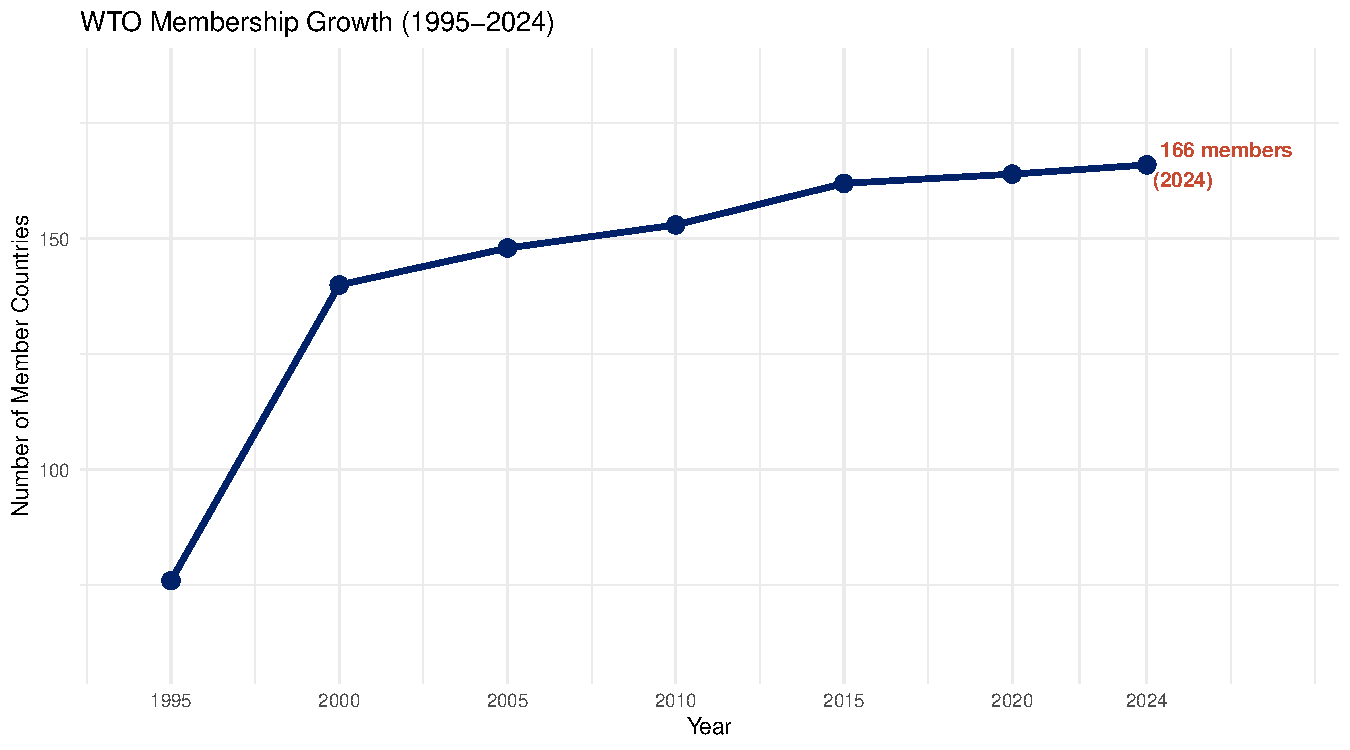
\includegraphics[keepaspectratio]{Lecture13_WTO_files/figure-beamer/fig-wto-membership-1.pdf}}

}

\caption{\label{fig-wto-membership}WTO Membership Growth (1995-2024)
Source: WTO Secretariat.}

\end{figure}%
\end{frame}

\begin{frame}
\end{frame}

\section{WTO Principles}\label{wto-principles}

\begin{frame}{The Five Core Principles of the WTO}
\phantomsection\label{the-five-core-principles-of-the-wto}
\textbf{The WTO rulebook rests on five foundational pillars --- all
member commitments flow from these}

\begin{columns}[T]
\begin{column}{0.5\linewidth}
\textbf{1. Most Favoured Nation (MFN)} Non-discrimination among all
members: a concession given to one must be given to all. \emph{Art. I
GATT, Art. II GATS}

\textbf{2. National Treatment} Imported goods must be treated no less
favourably than domestic goods \textbf{once inside the border}.
\emph{Art. III GATT}

\textbf{3. Bound Tariffs} Members commit to ceiling tariff rates (bound
rates) in their schedules --- cannot raise above without compensation.
\end{column}

\begin{column}{0.5\linewidth}
\textbf{4. Reciprocity} Concessions are exchanged mutually --- no free
riding. Basis of negotiating rounds.

\textbf{5. Transparency} Members must notify laws, regulations, and
trade measures to the WTO. No hidden barriers.

\textbf{Why these matter for India:} India's bound tariff schedule gives
it enormous policy space (bound 113\% average on agriculture vs.~applied
\textasciitilde35\%). These principles simultaneously protect India from
arbitrary foreign barriers.
\end{column}
\end{columns}
\end{frame}

\begin{frame}{MFN in Depth: The India Example}
\phantomsection\label{mfn-in-depth-the-india-example}
\begin{columns}[T]
\begin{column}{0.55\linewidth}
\textbf{How MFN Works}

If India gives the USA a \textbf{0\% tariff on apples}, under MFN, India
must give \textbf{the same 0\% to ALL WTO members} --- Canada,
Australia, Chile, New Zealand, China.

You cannot discriminate between WTO members.

\textbf{Permitted Exceptions:}

\begin{enumerate}
\tightlist
\item
  \textbf{Free Trade Agreements (Art. XXIV GATT):} Deeper preferences
  within FTA --- WTO legal if the FTA covers ``substantially all trade''
\item
  \textbf{GSP (Enabling Clause):} Developed countries can give
  preferential rates to developing countries unilaterally
\item
  \textbf{Security exceptions (Art. XXI):} National security
  justifications
\end{enumerate}
\end{column}

\begin{column}{0.45\linewidth}
\textbf{India's FTA Example}

India--UAE CEPA (2022): - India gives 0\% tariff on many UAE goods - WTO
members do NOT automatically get this rate - WTO-legal because CEPA is
an FTA under Art. XXIV

But India must ensure CEPA covers substantially all trade --- otherwise
challenged at WTO

\textbf{India's FTA network} (2024): UAE, Mauritius, Japan, South Korea,
ASEAN, Singapore, Sri Lanka, Thailand (partial), Australia, EFTA
\end{column}
\end{columns}
\end{frame}

\begin{frame}[fragile]{WTO Organisational Structure}
\phantomsection\label{wto-organisational-structure}
\begin{verbatim}
MINISTERIAL CONFERENCE  (Supreme body — every 2 years)
         │
   GENERAL COUNCIL  (Day-to-day — Geneva ambassadors)
    ┌────┴────────────────────────┐
    │                             │
Trade Policy Review Body    Dispute Settlement Body (DSB)
    │
    ├── Council for Trade in GOODS (GATT)
    │       ├── Committee on Agriculture
    │       ├── SPS Committee
    │       ├── TBT Committee
    │       ├── Anti-Dumping Committee
    │       └── Safeguards Committee
    │
    ├── Council for Trade in SERVICES (GATS)
    │
    └── Council for TRIPS
\end{verbatim}

\textbf{India's Geneva Mission} maintains a permanent delegation of
\textasciitilde30 diplomats/trade negotiators to engage all WTO bodies.
India chairs or co-chairs several committees.
\end{frame}

\begin{frame}{Ministerial Conferences: Key Milestones}
\phantomsection\label{ministerial-conferences-key-milestones}
\begin{columns}[T]
\begin{column}{0.5\linewidth}
\begin{longtable}[]{@{}
  >{\raggedright\arraybackslash}p{(\linewidth - 6\tabcolsep) * \real{0.1212}}
  >{\raggedright\arraybackslash}p{(\linewidth - 6\tabcolsep) * \real{0.3030}}
  >{\raggedright\arraybackslash}p{(\linewidth - 6\tabcolsep) * \real{0.1818}}
  >{\raggedright\arraybackslash}p{(\linewidth - 6\tabcolsep) * \real{0.3939}}@{}}
\toprule\noalign{}
\begin{minipage}[b]{\linewidth}\raggedright
MC
\end{minipage} & \begin{minipage}[b]{\linewidth}\raggedright
Location
\end{minipage} & \begin{minipage}[b]{\linewidth}\raggedright
Year
\end{minipage} & \begin{minipage}[b]{\linewidth}\raggedright
Key Outcome
\end{minipage} \\
\midrule\noalign{}
\endhead
MC1 & Singapore & 1996 & ``Singapore issues'': investment, competition,
procurement \\
MC3 & Seattle & 1999 & \textbf{Failed} --- ``Battle of Seattle'' \\
MC4 & \textbf{Doha} & 2001 & Launched Doha Development Agenda \\
MC5 & Cancún & 2003 & \textbf{Failed} --- G-20 coalition walked out \\
MC6 & Hong Kong & 2005 & Partial agriculture framework \\
\bottomrule\noalign{}
\end{longtable}
\end{column}

\begin{column}{0.5\linewidth}
\begin{longtable}[]{@{}llll@{}}
\toprule\noalign{}
MC & Location & Year & Key Outcome \\
\midrule\noalign{}
\endhead
MC9 & \textbf{Bali} & 2013 & \textbf{TFA + Peace Clause} \\
MC10 & \textbf{Nairobi} & 2015 & Export subsidy elimination \\
MC11 & Buenos Aires & 2017 & No consensus \\
MC12 & \textbf{Geneva} & 2022 & \textbf{Fisheries subsidies} \\
MC13 & Abu Dhabi & 2024 & E-commerce moratorium extended \\
\bottomrule\noalign{}
\end{longtable}

\textbf{India hosted MC6 in Hong Kong context} and has been central to
the G-33 and G-20 agricultural coalitions at every MC
\end{column}
\end{columns}
\end{frame}

\begin{frame}{Key WTO Agreements --- Overview}
\phantomsection\label{key-wto-agreements-overview}
\begin{columns}[T]
\begin{column}{0.5\linewidth}
\begin{longtable}[]{@{}
  >{\raggedright\arraybackslash}p{(\linewidth - 2\tabcolsep) * \real{0.4231}}
  >{\raggedright\arraybackslash}p{(\linewidth - 2\tabcolsep) * \real{0.5769}}@{}}
\toprule\noalign{}
\begin{minipage}[b]{\linewidth}\raggedright
Agreement
\end{minipage} & \begin{minipage}[b]{\linewidth}\raggedright
What it covers
\end{minipage} \\
\midrule\noalign{}
\endhead
\textbf{AoA} & Agriculture: market access, domestic support, export
subsidies \\
\textbf{SPS} & Food safety, animal \& plant health measures \\
\textbf{TBT} & Product standards, labelling, testing procedures \\
\textbf{Anti-Dumping} & Duties against below-cost imports \\
\textbf{SCM} & Subsidies \& countervailing duties \\
\bottomrule\noalign{}
\end{longtable}
\end{column}

\begin{column}{0.5\linewidth}
\begin{longtable}[]{@{}ll@{}}
\toprule\noalign{}
Agreement & What it covers \\
\midrule\noalign{}
\endhead
\textbf{Safeguards} & Emergency import restrictions \\
\textbf{GATS} & Trade in services (banking, telecom, education) \\
\textbf{TRIPS} & Intellectual property rights \\
\textbf{TFA} & Customs procedures, border facilitation \\
\textbf{Fisheries} & Subsidies for fishing fleets \\
\bottomrule\noalign{}
\end{longtable}

\textbf{For agricultural trade}, the most important are: AoA, SPS, TBT,
Anti-Dumping, and SCM. Lectures 14--16 cover these in depth.
\end{column}
\end{columns}
\end{frame}

\begin{frame}{Dispute Settlement Understanding (DSU)}
\phantomsection\label{dispute-settlement-understanding-dsu}
\textbf{WTO's most important institutional innovation} --- binding,
rules-based dispute resolution replacing GATT's ``diplomatic'' process

\begin{columns}[T]
\begin{column}{0.55\linewidth}
\textbf{The DSU Process:}

\begin{enumerate}
\tightlist
\item
  \textbf{Consultations} (60 days) --- bilateral negotiation
\item
  \textbf{Panel established} --- 3 trade law experts, 6--9 months
\item
  \textbf{Panel Report} adopted by DSB
\item
  \textbf{Appellate Body} --- 3 of 7 members, 60--90 days
\item
  \textbf{DSB adoption} --- quasi-automatic (reverse consensus)
\item
  \textbf{Implementation} --- reasonable time period
\item
  \textbf{Retaliation} --- if not complied, winning party can suspend
  concessions
\end{enumerate}
\end{column}

\begin{column}{0.45\linewidth}
\textbf{Appellate Body Crisis}

Since 2017, the \textbf{USA has blocked appointments} to the AB ---
currently non-functional (needs 3 members, has 0 active).

\textbf{MPIA:} Multi-Party Interim Appeal Arbitration Arrangement --- 53
members (including India) agreed to use arbitration as workaround.

USA objects: AB ``overreached'' its mandate by creating precedents.
\end{column}
\end{columns}
\end{frame}

\begin{frame}{India in WTO Disputes}
\phantomsection\label{india-in-wto-disputes}
\begin{columns}[T]
\begin{column}{0.5\linewidth}
\textbf{As Complainant (India won):}

\textbf{DS456 --- US-India Solar Cells (2016)} USA's domestic content
requirements for solar panels under the National Solar Mission violated
WTO national treatment (Art. III). India won --- US had to remove
requirements.

\textbf{Other active cases India initiated:} challenges to US steel
tariffs, EU carbon measures
\end{column}

\begin{column}{0.5\linewidth}
\textbf{As Respondent (India lost/challenging):}

\begin{itemize}
\tightlist
\item
  \textbf{DS265} --- EC-India Sugar Subsidies: India's sugar export
  subsidies found WTO-illegal; India appealing
\item
  \textbf{DS430} --- India-Agricultural Products: US challenged India's
  avian influenza ban on US poultry --- India lost on SPS grounds
\item
  \textbf{DS582} --- India-IT Tariffs: EU/Japan challenged India's IT
  product tariffs --- India lost
\item
  \textbf{DS541} --- India-MEIS: US challenged India's export incentive
  scheme --- India lost
\end{itemize}

India has participated in \textbf{50+ disputes} as complainant,
respondent, or third party --- reflecting deep WTO engagement
\end{column}
\end{columns}
\end{frame}

\begin{frame}{India's WTO Dispute Cases by Partner}
\phantomsection\label{indias-wto-dispute-cases-by-partner}
\begin{figure}

\centering{

\pandocbounded{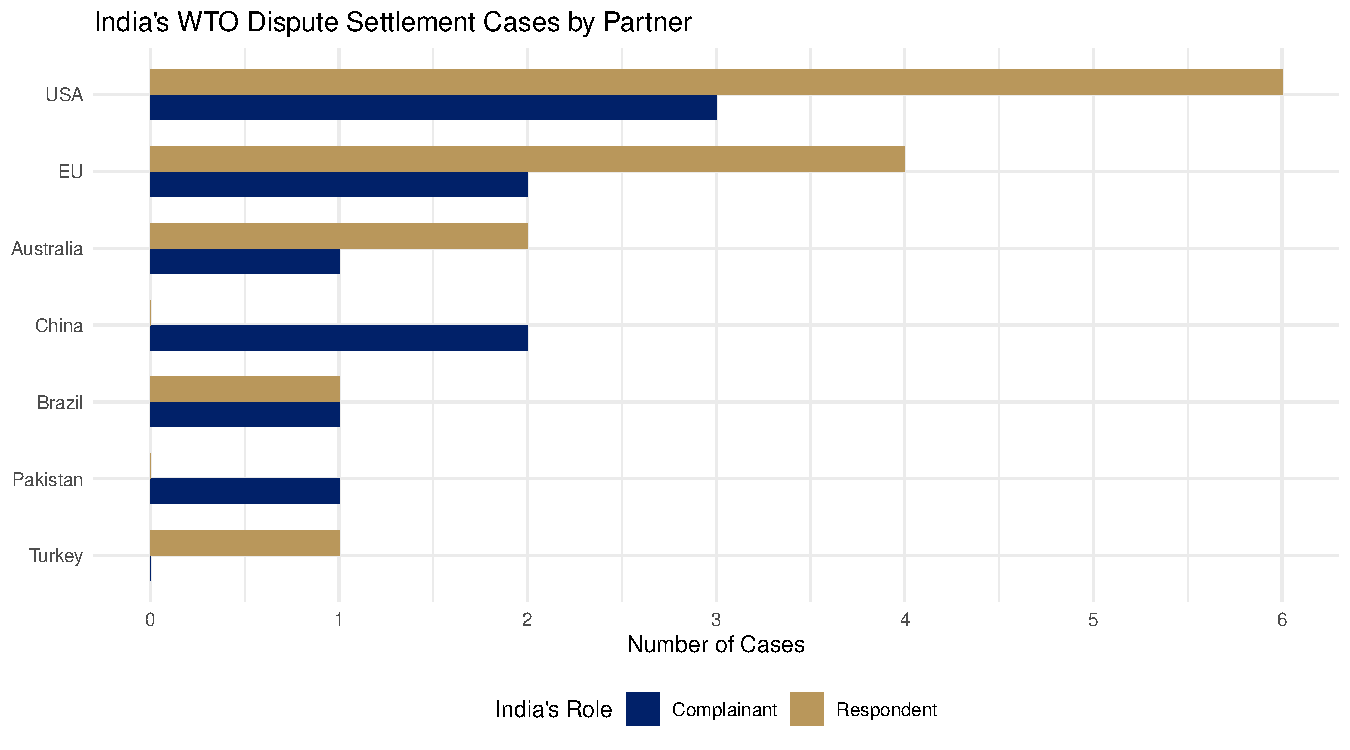
\includegraphics[keepaspectratio]{Lecture13_WTO_files/figure-beamer/fig-india-wto-disputes-1.pdf}}

}

\caption{\label{fig-india-wto-disputes}India's WTO Dispute Settlement
Cases by Partner Source: WTO Dispute Settlement Gateway (as of 2024).}

\end{figure}%
\end{frame}

\begin{frame}{India's WTO Negotiating Coalitions}
\phantomsection\label{indias-wto-negotiating-coalitions}
\begin{columns}[T]
\begin{column}{0.55\linewidth}
\textbf{India leads or co-leads multiple developing country coalitions:}

\textbf{G-33 (Chair: Indonesia, India active)} 46 developing countries.
Demands: Special Products (SP) --- exempt sensitive crops from tariff
cuts; Special Safeguard Mechanism (SSM) --- emergency tariff response to
import surges.

\textbf{G-20 Agricultural Group (India, Brazil, China, South Africa)}
Demands deep cuts in US/EU trade-distorting domestic support; improved
market access; elimination of export subsidies. \textbf{Not to be
confused with G20 heads of state summit.}

\textbf{NAMA-11:} Developing country coalition on industrial tariff
negotiations --- resist deep cuts.
\end{column}

\begin{column}{0.45\linewidth}
\textbf{Why Coalitions Matter}

WTO operates by \textbf{consensus} --- no voting for most decisions.
Coalitions give developing countries blocking power.

\textbf{India's G-33 Asks:} - 1.5 billion farmers in developing
countries need protection from import surges - Special Products: food
security crops (rice, wheat, pulses) protected from tariff cuts - SSM:
right to raise tariffs temporarily if imports surge and hurt local
farmers

India has successfully used these coalitions to block unfavourable
outcomes at Cancún (2003) and other MCs.
\end{column}
\end{columns}
\end{frame}

\begin{frame}{The Doha Development Round}
\phantomsection\label{the-doha-development-round}
\textbf{Launched:} November 2001, Doha, Qatar --- framed as a
``development round'' post-9/11 solidarity

\begin{columns}[T]
\begin{column}{0.55\linewidth}
\textbf{The Doha Agenda:}

\begin{itemize}
\tightlist
\item
  \textbf{Agriculture:} deep cuts in US/EU domestic support; improved
  market access; eliminate export subsidies
\item
  \textbf{Industrial goods (NAMA):} significant tariff cuts
\item
  \textbf{Services (GATS):} further liberalisation
\item
  \textbf{TRIPS \& Public Health:} access to medicines for poor
  countries
\item
  \textbf{Development:} special and differential treatment (S\&DT)
  strengthened
\end{itemize}

\textbf{Why it stalled --- the political economy:} - USA: Farm Bill
politics, Congress won't cut subsidies - EU: defensive on sugar, dairy,
beef - India/China: demand strong SSM for agriculture; resist industrial
tariff cuts (NAMA)
\end{column}

\begin{column}{0.45\linewidth}
\textbf{July 2008 Mini-Ministerial --- The Collapse}

India's then-Commerce Minister \textbf{Kamal Nath} walked out over SSM
provisions. The US wanted an import surge threshold of 140\% of base;
India demanded 110\%. Talks collapsed.

Symbolically important: India prioritised \textbf{farmer protection over
deal}.

Doha Round is effectively \textbf{dead as a single undertaking}. Some
elements (TFA, fisheries subsidies, export subsidy elimination) have
been harvested. The agriculture agenda --- the core --- remains
unresolved after 23+ years.
\end{column}
\end{columns}
\end{frame}

\begin{frame}{Trade Facilitation Agreement (TFA, 2017)}
\phantomsection\label{trade-facilitation-agreement-tfa-2017}
\begin{columns}[T]
\begin{column}{0.55\linewidth}
\textbf{First multilateral agreement fully concluded at WTO} --- in
force February 22, 2017

\textbf{Key provisions:} - \textbf{Advance rulings} on tariff
classification and origin - \textbf{Single window} for customs clearance
- \textbf{Expedited release} of perishable goods - \textbf{Risk-based
inspection} (not 100\% physical checks) - \textbf{Transit facilitation}
for landlocked countries - \textbf{Appeal procedures} for customs
decisions

\textbf{Benefits for India's agri exports:} Perishables (mangoes,
grapes, vegetables) need fast clearance. TFA obliges importing countries
to have expedited procedures.
\end{column}

\begin{column}{0.45\linewidth}
\textbf{India's TFA Implementation:}

\begin{itemize}
\tightlist
\item
  \textbf{ICEGATE} single window for customs
\item
  24/7 operations at major ports
\item
  Risk-based inspection system (SWIFT)
\item
  Authorised Economic Operator (AEO) programme
\end{itemize}

\textbf{Time Release Study (India):}

\begin{longtable}[]{@{}lll@{}}
\toprule\noalign{}
Channel & Before & After TFA \\
\midrule\noalign{}
\endhead
Air cargo & 120 hrs & \textbf{49 hrs} \\
Sea cargo & 180 hrs & \textbf{68 hrs} \\
\bottomrule\noalign{}
\end{longtable}

World Bank estimates: full TFA implementation could reduce trade costs
by \textbf{14.3\%} for developing countries
\end{column}
\end{columns}
\end{frame}

\begin{frame}{WTO Fisheries Subsidies Agreement (MC12, 2022)}
\phantomsection\label{wto-fisheries-subsidies-agreement-mc12-2022}
\begin{columns}[T]
\begin{column}{0.55\linewidth}
\textbf{First new multilateral WTO agreement on fisheries subsidies}

\textbf{Prohibits:} - Subsidies for Illegal, Unreported, and Unregulated
(IUU) fishing - Subsidies for fishing overfished stocks - Subsidies for
fishing in unregulated high seas

\textbf{Context:} \textasciitilde USD 22 billion/year in global
fisheries subsidies; fishing stocks critically depleted --- 34\%
overfished globally

\textbf{Developing country flexibilities:} - Transition period of 2
years for some provisions - Inshore fishing (within 12 nautical miles)
largely exempted - LDCs: longer transitions
\end{column}

\begin{column}{0.45\linewidth}
\textbf{India's Position and Interests}

India's concerns: - Protect \textbf{small-scale traditional fishermen}
(Kerala, Tamil Nadu, Andhra Pradesh coastal communities) - India's
fishing subsidies (fuel subsidy, boat building) support livelihood of
\textasciitilde14 million fishers - Demand: developed country
distant-water fleets (EU, China, Japan) subsidised for decades --- they
caused the overfishing problem, not Indian small fishermen

India negotiated carve-outs for artisanal fishing within national EEZ
(200 nautical miles). Still under negotiation for full implementation.
\end{column}
\end{columns}
\end{frame}

\begin{frame}{WTO and India's Food Security Tension}
\phantomsection\label{wto-and-indias-food-security-tension}
\begin{columns}[T]
\begin{column}{0.5\linewidth}
\textbf{The Policy Conflict}

India's food security system: 1. \textbf{MSP} (Minimum Support Price)
set above world prices for wheat and rice 2. \textbf{FCI} procures at
MSP from farmers 3. \textbf{PDS} distributes at subsidised rates to poor
households

WTO critics argue: purchasing above world prices = \textbf{Amber Box
support} (trade-distorting domestic support) that must be counted
against India's AMS commitment

India's defence: The \textbf{Fixed External Reference Price (FERP)} used
to calculate AMS uses 1986--88 world prices --- which were artificially
depressed by US/EU subsidies at the time. The baseline is unfair.
\end{column}

\begin{column}{0.5\linewidth}
\textbf{The Numbers}

India's rice MSP (FY2024): \textbf{₹2,183/quintal}

FERP (1986--88): \textbf{USD 116/tonne = \textasciitilde USD
11.6/quintal}

Current MSP ≈ \textbf{USD 26.3/quintal}

AMS = (26.3 − 11.6) × 42 million tonnes procured ≈
\textbf{\textasciitilde USD 6.2 billion}

De minimis limit (10\% of rice production) ≈ \textbf{\textasciitilde USD
2.8 billion}

→ India likely exceeds its de minimis threshold → \textbf{Peace Clause
protection needed}
\end{column}
\end{columns}
\end{frame}

\begin{frame}{The Peace Clause (Bali, 2013)}
\phantomsection\label{the-peace-clause-bali-2013}
\begin{columns}[T]
\begin{column}{0.55\linewidth}
\textbf{Agreement on Public Stockholding for Food Security}

Bali MC9 (December 2013) --- negotiated primarily by \textbf{India}
under Commerce Minister Anand Sharma

\textbf{Protection offered:} WTO members will not formally challenge
developing country public stockholding programs even if they technically
exceed de minimis AMS limits, \textbf{provided:}

\begin{enumerate}
\tightlist
\item
  Program existed before December 2013
\item
  Regular, detailed notifications to the WTO Committee on Agriculture
\item
  Stocks not released onto world markets at below-market prices
\item
  Programme targeted at traditional staple foods and the poor
\end{enumerate}

India notifies rice, wheat, and coarse cereal procurement every year
under the Peace Clause.
\end{column}

\begin{column}{0.45\linewidth}
\textbf{The Catch}

\begin{itemize}
\tightlist
\item
  Agreed as \textbf{interim measure} pending permanent solution
\item
  Nairobi MC10 (2015): committed to finding permanent solution by MC11
  (2017) --- missed
\item
  Permanent solution still \textbf{not agreed} as of 2024 despite every
  MC discussing it
\item
  India's position: permanent solution must include new FERP methodology
\end{itemize}

The Peace Clause is India's single most important WTO negotiating
achievement in recent years. Without it, India's PDS + FCI procurement
system would be legally vulnerable to challenge.
\end{column}
\end{columns}
\end{frame}

\begin{frame}{TRIPS and Indian Agriculture}
\phantomsection\label{trips-and-indian-agriculture}
\begin{columns}[T]
\begin{column}{0.55\linewidth}
\textbf{TRIPS Agreement (1995):} Patents, copyrights, trademarks,
geographical indications, and plant variety protection.

\textbf{Key tension for agriculture:} TRIPS Art. 27.3(b) requires
protection of plant varieties either through patents or a sui generis
system.

\textbf{India's response --- PPVFRA (2001):} Protection of Plant
Varieties and Farmers' Rights Act --- India's sui generis system

\textbf{Key PPVFRA provisions:} - \textbf{Breeders' rights:} 15--18
years protection for new varieties - \textbf{Farmers' right:} to save,
use, sow, re-sow, exchange, and sell farm-saved seed (CANNOT sell under
breeder's brand) - \textbf{Researchers' exemption:} use protected
variety for research/breeding - \textbf{National Gene Fund:}
benefit-sharing from commercialisation
\end{column}

\begin{column}{0.45\linewidth}
\textbf{Monsanto Bt Cotton Case}

Monsanto held trait patent on Bt cotton gene in India. Charged royalties
(trait value) to all seed companies using the Bt technology.

India's seed companies: royalties too high, technology should be
accessible.

2021: Supreme Court ruled plant varieties and essentially biological
processes are \textbf{not patentable} under Indian Patents Act Section
3(j).

Monsanto's patent on Bt gene effectively invalidated in India.

India resists \textbf{TRIPS-plus} obligations pushed in FTA negotiations
(longer patent terms, data exclusivity for agrochem companies) that
would restrict farmer seed access
\end{column}
\end{columns}
\end{frame}

\begin{frame}{India's WTO Schedules and Policy Space}
\phantomsection\label{indias-wto-schedules-and-policy-space}
\begin{columns}[T]
\begin{column}{0.5\linewidth}
\textbf{India's Bound Tariff Schedule --- Agriculture}

\begin{longtable}[]{@{}llll@{}}
\toprule\noalign{}
Commodity & Bound & Applied (2024) & ``Water'' \\
\midrule\noalign{}
\endhead
Rice & 80\% & 25\% & 55\% \\
Wheat & 100\% & 40\% & 60\% \\
Maize & 60\% & 50\% & 10\% \\
Sugar & 150\% & 100\% & 50\% \\
Palm oil & 300\% & 100\% & 200\% \\
Milk powder & 60\% & 30\% & 30\% \\
\bottomrule\noalign{}
\end{longtable}

\textbf{Average bound tariff on agriculture: 113.5\%} \textbf{Average
applied tariff: \textasciitilde35\%}
\end{column}

\begin{column}{0.5\linewidth}
\textbf{The ``Water in the Tariff'' = Policy Space}

The gap between bound and applied tariffs means India can \textbf{raise
applied tariffs without WTO violation}. This is India's key defensive
instrument.

Example: When palm oil imports surged hurting domestic oilseed farmers,
India raised the applied tariff from 30\% to 100\% --- still below the
300\% bound rate. No WTO violation.

\textbf{AMS De Minimis:} 10\% of production value (developing country
rate --- vs.~5\% for developed). This is why India gets more space than
the US/EU.
\end{column}
\end{columns}
\end{frame}

\begin{frame}{Recent WTO Issues Affecting India}
\phantomsection\label{recent-wto-issues-affecting-india}
\begin{columns}[T]
\begin{column}{0.5\linewidth}
\textbf{E-Commerce Moratorium}

Since 1998: WTO members agreed no customs duties on \textbf{electronic
transmissions} (digital goods, streaming, software downloads).

Extended at every MC including MC13 (Abu Dhabi 2024).

\textbf{India's position:} End the moratorium. India loses potential
tariff revenue on digital goods (music, films, software, data). India
and South Africa are the most vocal opponents.

India argues: rich country digital companies benefit most; developing
countries lose fiscal revenue.
\end{column}

\begin{column}{0.5\linewidth}
\textbf{Joint Statement Initiatives (JSIs)}

Plurilateral negotiations outside the main WTO consensus framework: -
E-commerce JSI (90 members) - Investment facilitation JSI - Domestic
regulation (services)

\textbf{India did NOT join} the e-commerce JSI or investment
facilitation JSI.

India's concern: JSI outcomes should not become part of WTO multilateral
rules without consensus of all 166 members.

Reflects India's \textbf{defensive posture} on digital trade --- India
wants to preserve policy space to regulate data and digital economy.
\end{column}
\end{columns}
\end{frame}

\begin{frame}{Key Takeaways: WTO}
\phantomsection\label{key-takeaways-wto}
\textbf{Six Things to Remember from Lecture 13}

\begin{enumerate}
\item
  \textbf{WTO replaced GATT on Jan 1, 1995} --- the Uruguay Round
  (1986--94) was the turning point; 166 members, India a founding member
\item
  \textbf{Five core principles:} MFN, National Treatment, Bound Tariffs,
  Reciprocity, Transparency --- these are the rules of the game
\item
  \textbf{DSU is WTO's crown jewel} --- binding dispute settlement;
  India has won and lost important cases; Appellate Body crisis
  unresolved
\item
  \textbf{Doha Round is effectively dead} --- agriculture at the centre
  of the stalemate; US/EU domestic politics vs.~India/developing country
  demands
\item
  \textbf{Peace Clause (2013) is India's lifeline} --- protects
  MSP-based procurement from WTO challenge; permanent solution still
  pending
\item
  \textbf{India uses WTO strategically:} high bound tariffs for policy
  space, G-33/G-20 coalitions for negotiating power, DSU for defending
  interests
\end{enumerate}
\end{frame}

\begin{frame}{Next Lecture: Agreement on Agriculture}
\phantomsection\label{next-lecture-agreement-on-agriculture}
\begin{columns}[T]
\begin{column}{0.6\linewidth}
\textbf{Lecture 14 (July 28, 2026):}

\textbf{Agreement on Agriculture (AoA)}

The WTO agreement that \textbf{directly governs India's agricultural
trade policy}

We will cover:

\begin{itemize}
\tightlist
\item
  \textbf{Three Pillars} in depth: Market Access, Domestic Support,
  Export Competition
\item
  Tariffication and Tariff Rate Quotas
\item
  The Three Boxes: Green, Blue, Amber
\item
  India's AMS challenge --- the numbers
\item
  The Peace Clause revisited in technical detail
\item
  India's export subsidy constraints
\item
  Special and Differential Treatment
\end{itemize}
\end{column}

\begin{column}{0.4\linewidth}
\textbf{Prepare for Lecture 14:}

Think about this question:

\emph{``India provides fertiliser subsidies worth ₹2.25 lakh crore per
year. Is this WTO-legal? Which `box' does it fall in?''}

We will work through the answer systematically using the AoA framework.

\textbf{Reading:} - WTO Agreement on Agriculture (full text --- 35
pages) - CUTS International: \emph{India and WTO Agriculture
Negotiations} (2023) - Economic Survey 2023-24, Chapter on Agriculture
\end{column}
\end{columns}
\end{frame}

\section{Appendix}\label{appendix}

\begin{frame}{Additional Resources}
\phantomsection\label{additional-resources}
\begin{columns}[T]
\begin{column}{0.5\linewidth}
\textbf{Further Reading}

\begin{itemize}
\tightlist
\item
  \emph{International Economics} --- Salvatore (Ch. 12)
\item
  \emph{International Economics} --- Appleyard \& Field (Ch. 12)
\item
  RBI/DGCI\&S/APEDA databases for latest data
\end{itemize}
\end{column}

\begin{column}{0.5\linewidth}
\textbf{Key Data Sources}

\begin{itemize}
\tightlist
\item
  DGCI\&S: India's merchandise trade
\item
  RBI: Balance of payments data\\
\item
  APEDA: Agricultural export statistics
\item
  WTO: Tariff and trade databases
\end{itemize}
\end{column}
\end{columns}
\end{frame}




\end{document}
